\chapter{FAHP多维资源建模和参数自动求解}
在上一节新的评分函数中,根据资源的重要程度使用\begin{math}\alpha_{i}(i=1,2,3,4,5),  alpha_{1}+\alpha_{2}+\alpha_{3}+\alpha_{4}+\alpha_{5}=1\end{math}作为CPU、内存、磁盘I/O、网络带宽和已部署Pod数量的重要程度系数。本章需要对预选筛选后的节点资源进行建模,并利用FAHP方法进行调度Pod多维权重参数的自动求解。

\section{模糊层次分析法FAHP}
模糊层次分析法FAHP(Fuzzy Analytical Hierarchy Process)是在层次分析法的基础发展而来,常用于解决实际问题中影响决策问题的多种因素的权重。下面从层次分析法开始介绍,为弥补层次分析法的不足引入FAHP方法,然后举例说明如何使用该方法解决实际问题。

\subsection{FAHP方法介绍}
在面对许多实际问题解决方案时,我们往往需要对影响方案的因素进行比较、判断、评价,然后做出决策,这种人工主观解决问题的方式不但效率低下,结果也不够准确。层析分析法(Analytical Hierarchy Process)是由著名的美国运筹学家匹茨堡大学T.L.Saaty教授提出的一种层次权重决策分析方法。该方法用于解决复杂的多目标决策问题,将影响目标决策的因素分解为目标层、准则层和方案层等层次,使用数学方法对个因素进行精确求解。层次分析法将问题的总目标、各层子目标以及决策因素分解成多个层次结构,然后构建各层次的判断矩阵,求解判断矩阵的特征值。最大特征值对应的特征向量归一化获得本层各元素上一层次某元素的优先权重,最后再加权和的方法递阶归并各备择方案对总目标的最终权重,选择最终权重最大的方案作为选择的方案。该方法是一个系统性的分析方法,先将问题分解成多个层次,然后对影响子目标的因素进行比较判断、最终进行综合决策。结构层次清晰、单层的权重参数设置都会影响到最终的决策层,不断分割量化各因素的影响。层次分析法非常实用,将定量分析和定性分析相结合,解决许多实际问题如电力分配、旅游决策等,该方法计算简单明了,易于掌握。最后,该方法具有简洁性,用于模拟人们解决问题的思维,所需的定量信息较少,仅需要对影响决策因素的重要性做出判断即可。

但是,层次分析法也具有局限性,在一些场景下无法使用或者效果较差。首先,该方法只能从实际的备选方案中帮助决策者选出较优的决策方案,不能给决策者提供新的解决方案或者反馈合理方案的意见,此外,该方法是单目标决策方法,使用者只能选出一个最优的目标。其次,该方法模拟人类大脑决策过程,定性分析过于浓厚,只能进行粗略比较计算,不能完全做到精确模拟。最后,从层次结构转化为成对比矩阵过程中,判断者的主观因素影响过大,判断者不同,得出的最优方案也不尽相同,无法让人信服。并且随着影响决策因素的增加,构建的成对比矩阵阶数增大,计算难度和复杂度随之增加,很难一次性构建出满足一致性要求的成对比矩阵。

为减少人为主观因素对决策结果的影响,模糊层析分析法FAHP在层次分析法的基础上增加人为判断的模糊性,具体而言就是层析分析通过两两比较构建成对比判断矩阵,FAHP通过两两比较构建模糊成对比矩阵,提升了层次分析法解决问题的可靠性。在进行问题判断或专家咨询时,往往不是给出一个具体值,而是一个模糊数,如三值判断(最低可能值、最可能值和最大可能值)、二值区间等。下面先介绍模糊数集的概念,对于一个明确的集合:
\begin{equation}
\mu_{A}(x) = \left\{\begin{array}{l}
1, x\in A \\ [0.3cm]
0, x\notin A
\end{array}\right.
\end{equation}
明确的集合中,\begin{math}x\in A\end{math}时值为1,\begin{math}x\notin A\end{math}时值为0.但对于一个模糊数集,并不能完全明确x是否属于A,只能用[0,1]表示其隶属度。
\begin{equation}
\mu_{A}(x):U\to[0,1]
\end{equation}
\begin{math}\mu_{A}(x)\end{math}表示\begin{math}x\in A\end{math}的隶属度,也称\begin{math}\mu_{A}(x)\end{math}为集合A的隶属函数。对于任意的模糊数集,都对应一个隶属函数,隶属函数通常模仿概率论中的分布函数如正态分布、梯形分布、K次抛物线分布、S分布以及柯西分布等,值域在[0,1]上。

1983年,荷兰学者Van Loargoven首次提出用三角模糊数作为模糊数集的判断标准,并运用三角模糊数的运算和对数最小二乘法获取权重值。设论域R上的模糊数M为三角模糊数,M对应的隶属函数\begin{math}\mu_{M:}R\to[0,1]\end{math}满足下列函数:
\begin{equation}
\mu_{M}(x) = \left\{\begin{array}{l}
0 \quad x<a \\ [0.3cm]
\frac{x-a}{b-a} \quad a\le x\le b \\ [0.2cm]
\frac{c-x}{c-b} \quad b\le x\le c \\ [0.2cm]
0 \quad x>c
\end{array}\right.
\end{equation}
M=(a,b,c)其中\begin{math}a\le b\le c\end{math},
a和c分别表示三角模糊数的上界和下界值,b是隶属度为1的中间值,x=b时表示x完全属于M,在a和c之外的完全不属于模糊数M。定义一个置信度\begin{math}\alpha\end{math}可以将三元组的模糊数M化为一个\begin{math}\alpha\end{math}割集的二元形式,从而构建割集矩阵,设定优化参数后将二元值的矩阵转化成最终的判断矩阵。
\begin{equation}
	M_{\alpha} = [a^{\alpha},c^{\alpha}]=[(b-a)\alpha+a,-(c-b)\alpha+c] \quad \forall \alpha\in[0,1]
\end{equation}
根据Arnold J. Kaufmann在文献[xx]中的描述,\begin{math}\alpha\end{math}割集后的基本运算规则如下:
\begin{equation}
\begin{split}
	M_{\alpha} &= [m_{L}^{\alpha},m_{R}^{\alpha}] \\[0.2cm]
	N_{\alpha} &= [n_{L}^{\alpha},n_{R}^{\alpha}] \\[0.2cm]
	M_{\alpha}\oplus N_{\alpha} &= [m_{L}^{\alpha}+n_{L}^{\alpha},m_{R}^{\alpha}+n_{R}^{\alpha}] \\[0.2cm]
	M_{\alpha}\ominus N_{\alpha} &= [m_{L}^{\alpha}-n_{L}^{\alpha},m_{R}^{\alpha}-n_{R}^{\alpha}] \\[0.2cm]
	M_{\alpha}\otimes N_{\alpha} &= [m_{L}^{\alpha}n_{L}^{\alpha},m_{R}^{\alpha}n_{R}^{\alpha}] \\[0.2cm]
	M_{\alpha}\oslash N_{\alpha} &= [m_{L}^{\alpha}/n_{L}^{\alpha},m_{R}^{\alpha}/n_{R}^{\alpha}] \\[0.2cm]
	\end{split}
\end{equation}
本文采用三角模糊数进行FAHP的权重参数求解,并将三元组的M=(a,b,c)转化成\begin{math}\alpha\end{math}割集形式
\begin{math}M_{\alpha} =[(b-a)\alpha+a,-(c-b)\alpha+c] \quad \forall \alpha\in[0,1]\end{math}。

\subsection{FAHP求解权重参数步骤}
介绍完层次分析方法和模糊层析分析方法以及模糊数的基本概念后,下面用三角模糊数作为模糊程度的衡量值,FAHP求解权重参数步骤如下:
\begin{figure}[H] % use float package if you want it here
	\centering
	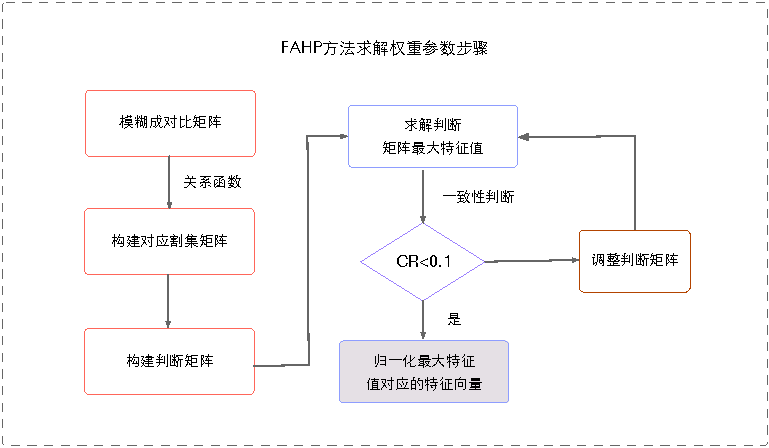
\includegraphics{fahp-flow}
	\caption{FAHP计算权重参数过程}
	\label{fig:xfig1}
\end{figure}











